\chapter{Testing Results}
\label{appendix:test_results}
This appendix chapter shows the different sections of the application that has been tested and the test outcomes.

%\section{Random Number Generator}

%The Bayes Durham Shuffle ensures that the psuedo random numbers used in the simulation are further shuffled, ensuring minimal correlation between subsequent random outputs \cite{NumericalRecipes}.

%\begin{verbatim}

%\end{verbatim}
\section{Unit tests}
\subsection{Binarise image}
\begin{figure}[H]
  \centering
  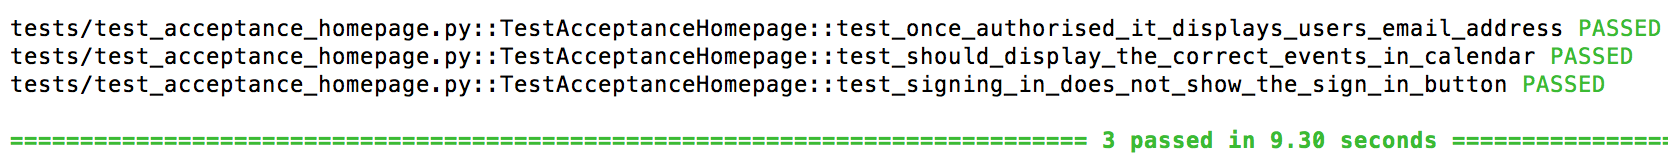
\includegraphics[width=\textwidth]{images/test_acceptance_homepage}
  \caption{Acceptance test being conducted for the homepage, to ensure that the homepage displays the correct content.}
  \label{fig:acceptance_homepage}
\end{figure}

\subsection{Calendar item}

\subsection{DateTimeHelper}


\section{Acceptance tests}
\label{appendix:acceptance}
The following section displays visual representation of the acceptance tests being executed, and their overall status.
\subsection{Homepage}

\begin{figure}[H]
  \centering
  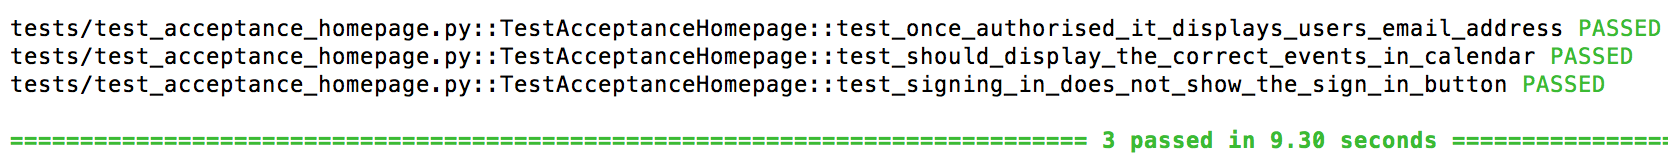
\includegraphics[width=\textwidth]{images/test_acceptance_homepage}
  \caption{Acceptance test being conducted for the homepage, to ensure that the homepage displays the correct content.}
  \label{fig:acceptance_homepage}
\end{figure}

\subsection{Add meta-data}

\begin{figure}[H]
  \centering
  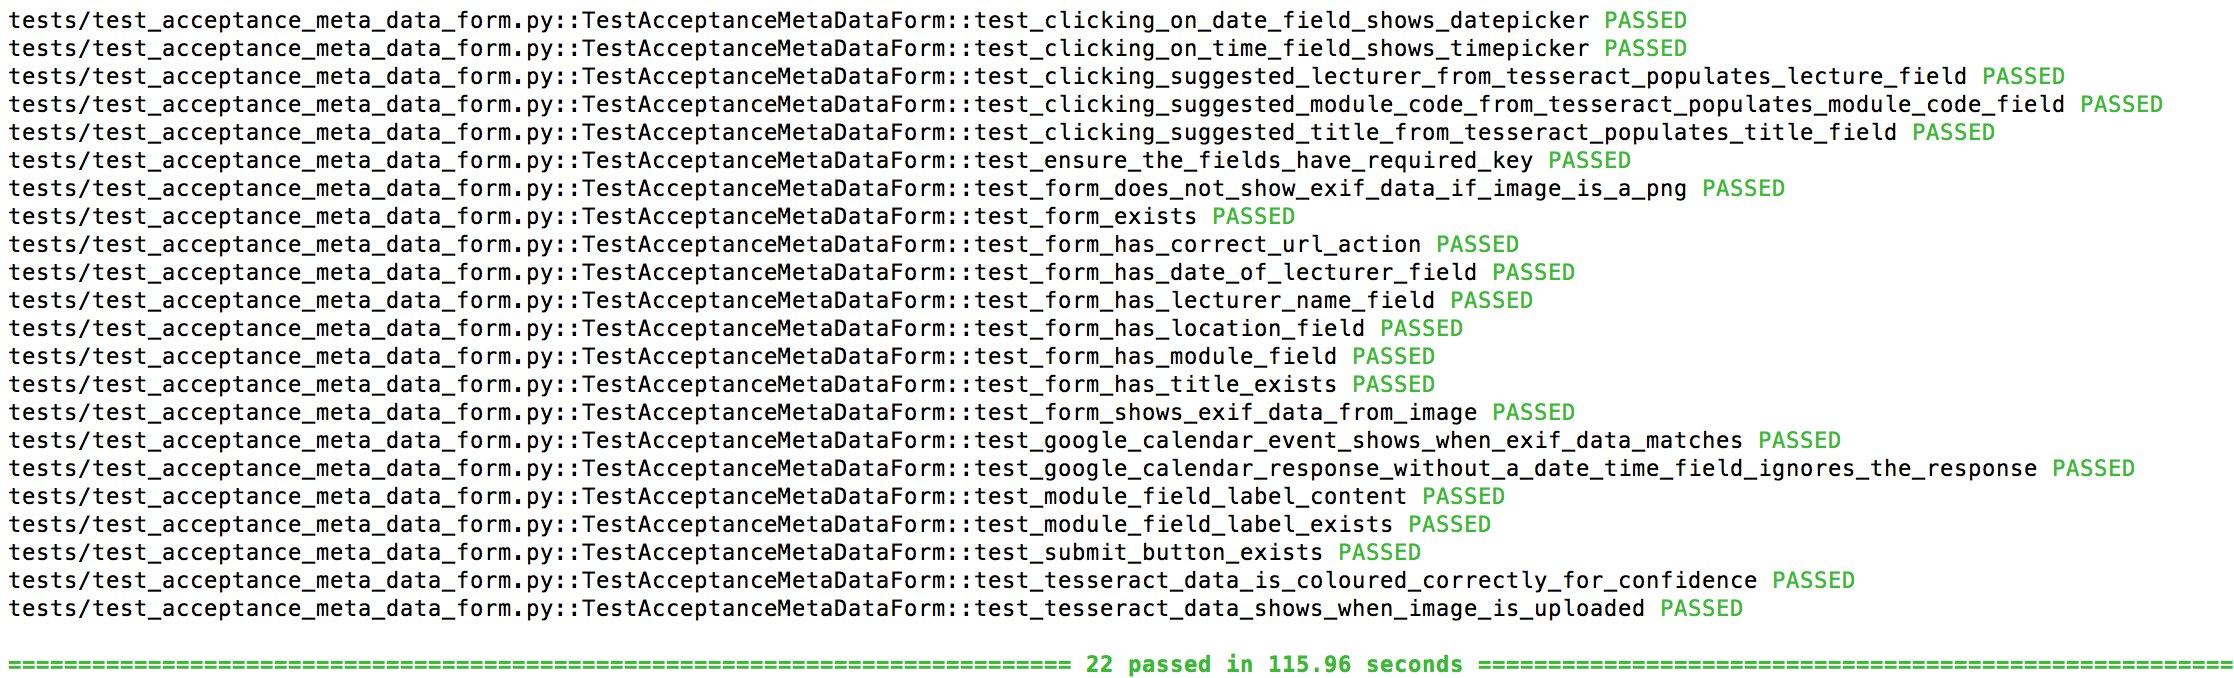
\includegraphics[width=\textwidth]{images/test_acceptance_meta_data_form}
  \caption{Acceptance test being performed to ensure that meta-data can be added to the correct note.}
  \label{fig:acceptance_add_meta_data}
\end{figure}

\subsection{Edit meta-data}
\begin{figure}[H]
  \centering
  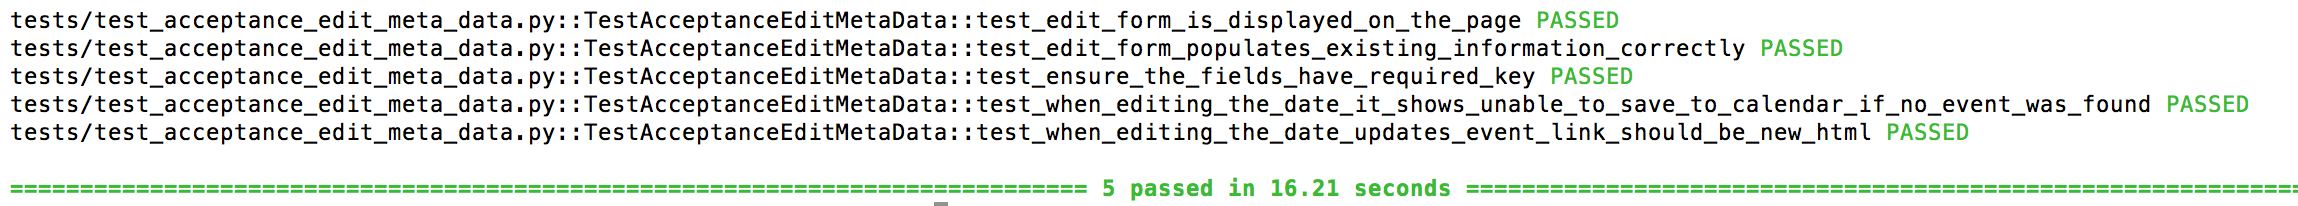
\includegraphics[width=\textwidth]{images/test_acceptance_edit_meta_data}
  \caption{Acceptance test being conducted so that a note's meta-data can be edited successfully.}
  \label{fig:acceptance_edit_meta_data}
\end{figure}
\subsection{Search}

\begin{figure}[H]
  \centering
  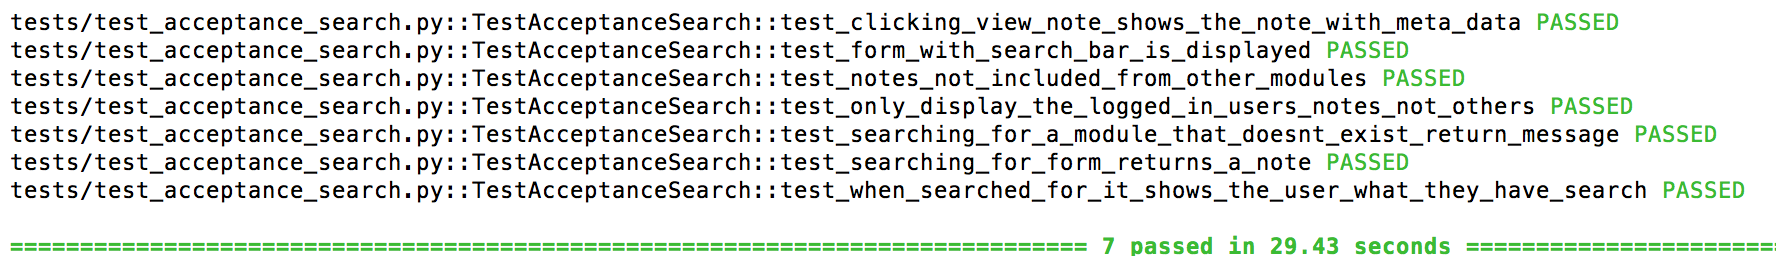
\includegraphics[width=\textwidth]{images/test_acceptance_search}
  \caption{Acceptance test to ensure that a user can search for a module code and it displays their notes.}
  \label{fig:search}
\end{figure}

\subsection{Viewing all the notes}

\begin{figure}[H]
  \centering
  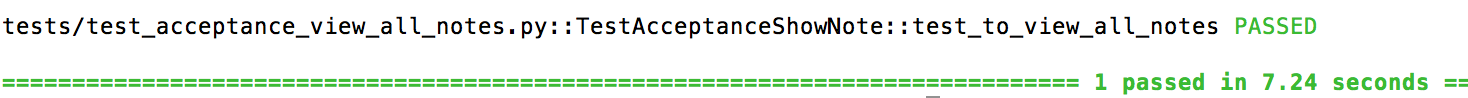
\includegraphics[width=\textwidth]{images/test_acceptance_view_notes}
  \caption{Acceptance test being conducted to ensure that all the notes can be viewed.}
  \label{fig:acceptance_view_note}
\end{figure}
\subsection{Show a note}

\begin{figure}[H]
  \centering
  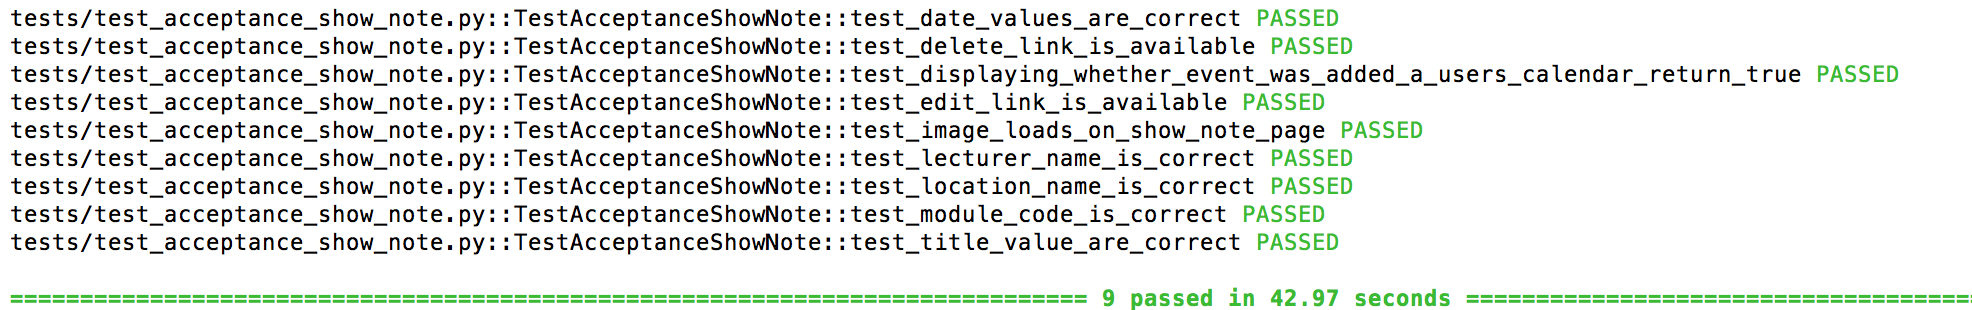
\includegraphics[width=\textwidth]{images/test_acceptance_show_note}
  \caption{Acceptance test being conducted to make sure that a singular note can be viewed correctly.}
  \label{fig:acceptance_homepage}
\end{figure}

\section{Integration tests}
\label{appendix:integration_tests}

\subsection{Add and edit meta data}
\begin{figure}[H]
  \centering
  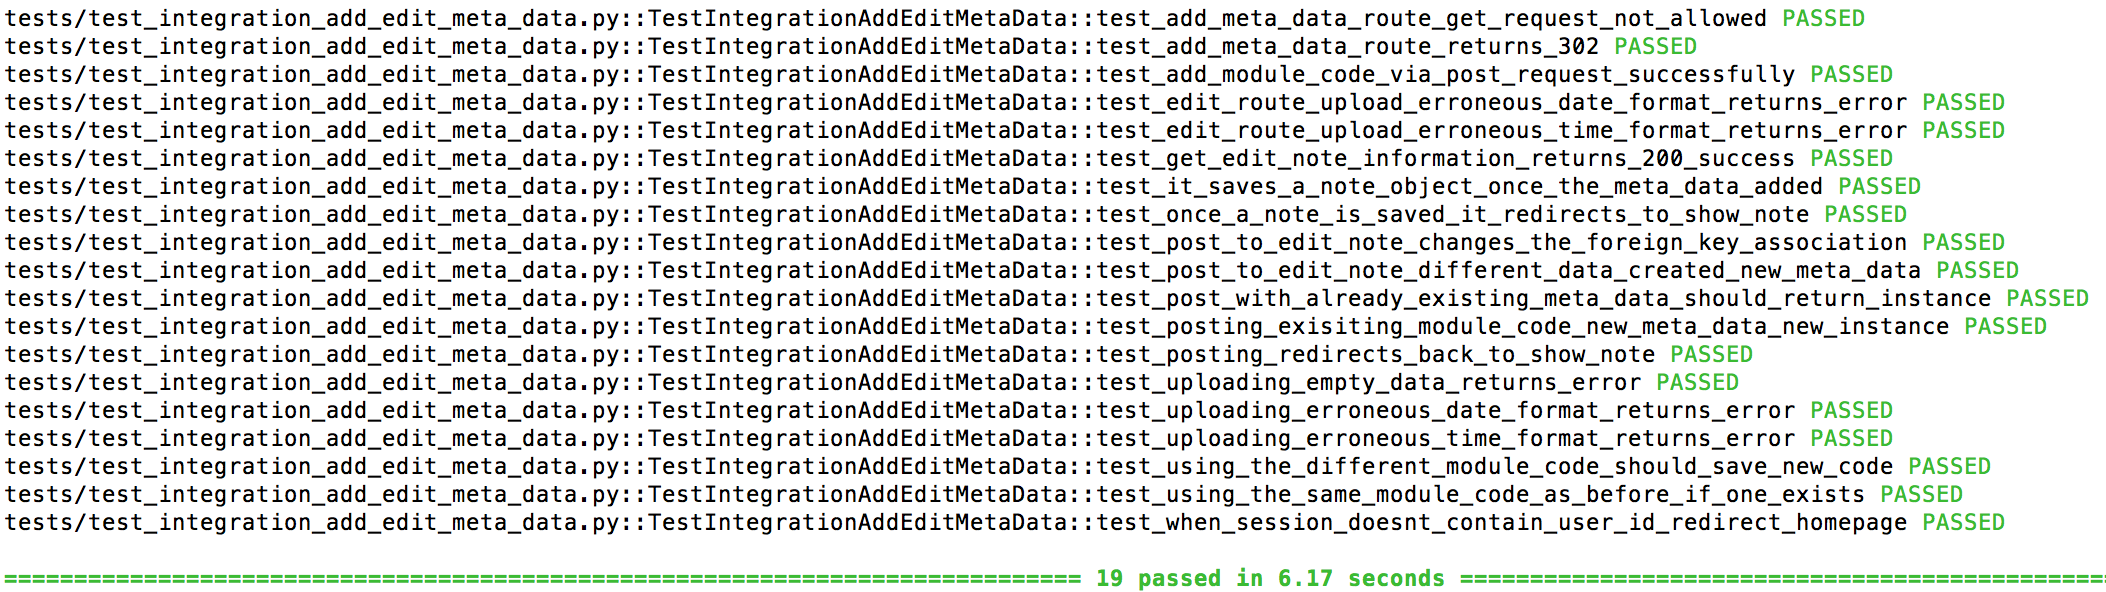
\includegraphics[width=\textwidth]{images/test_integration_add_edit_meta_data}
  \caption{Integration tests carried on the add and edit meta url to ensure the system worked well together.}
  \label{fig:integration_add_edit}
\end{figure}

\subsection{Homepage}
\begin{figure}[H]
  \centering
  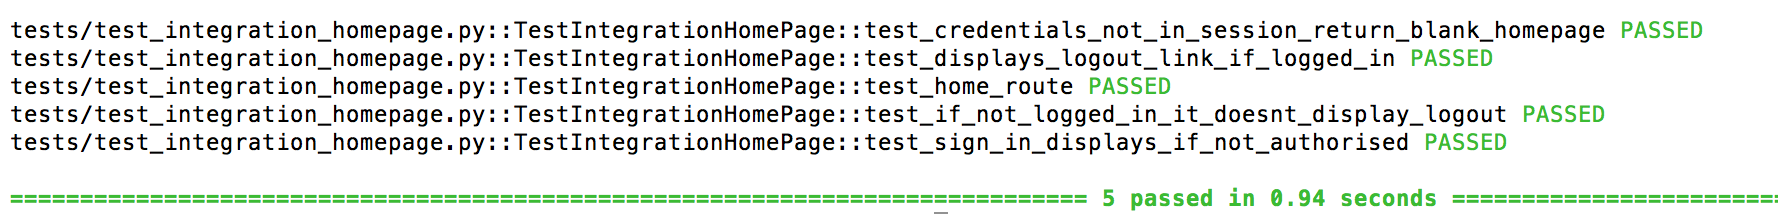
\includegraphics[width=\textwidth]{images/test_integration_homepage}
  \caption{Integration tests conducted on the homepage to ensure that the routes were accessible.}
  \label{fig:integration_homepage}
\end{figure}

\subsection{Logout}
\begin{figure}[H]
  \centering
  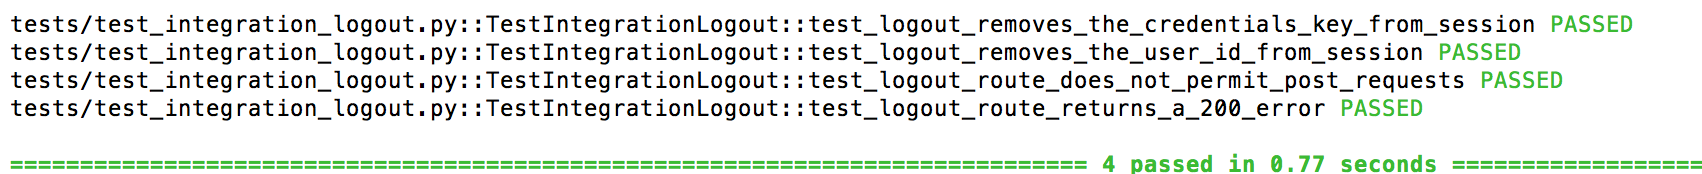
\includegraphics[width=\textwidth]{images/test_integration_logout}
  \caption{Integration tests conducted for the logout route ensuring the routes are logged out.}
  \label{fig:integration_logout}
\end{figure}

\subsection{Oauth}
\begin{figure}[H]
  \centering
  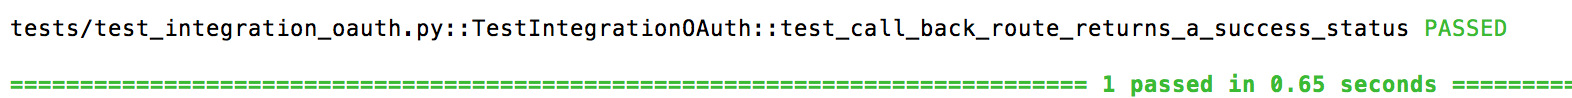
\includegraphics[width=\textwidth]{images/test_integration_oauth}
  \caption{Integration tests conducted for the oAuth route which interacts with the Google API.}
  \label{fig:integration_oauth}
\end{figure}

\subsection{Search}
\begin{figure}[H]
  \centering
  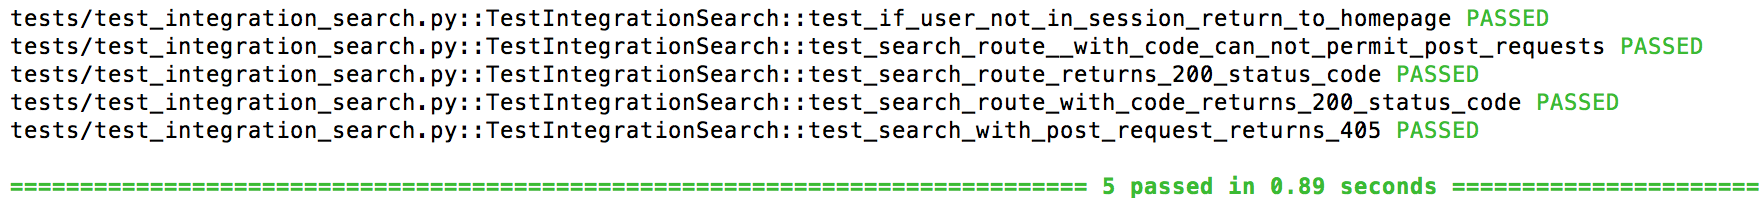
\includegraphics[width=\textwidth]{images/test_integration_search}
  \caption{Integration tests conducted for the search URL to ensure searching works correctly.}
  \label{fig:integration_search}
\end{figure}

\subsection{Show note}
\begin{figure}[H]
  \centering
  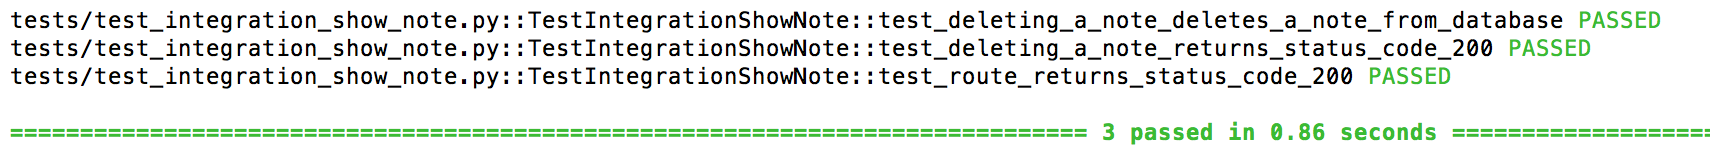
\includegraphics[width=\textwidth]{images/test_integration_show_note}
  \caption{Integration tests implemented to ensure that the note can be displayed properly. }
  \label{fig:integration_show_note}
\end{figure}

\section{Upload}
\begin{figure}[H]
  \centering
  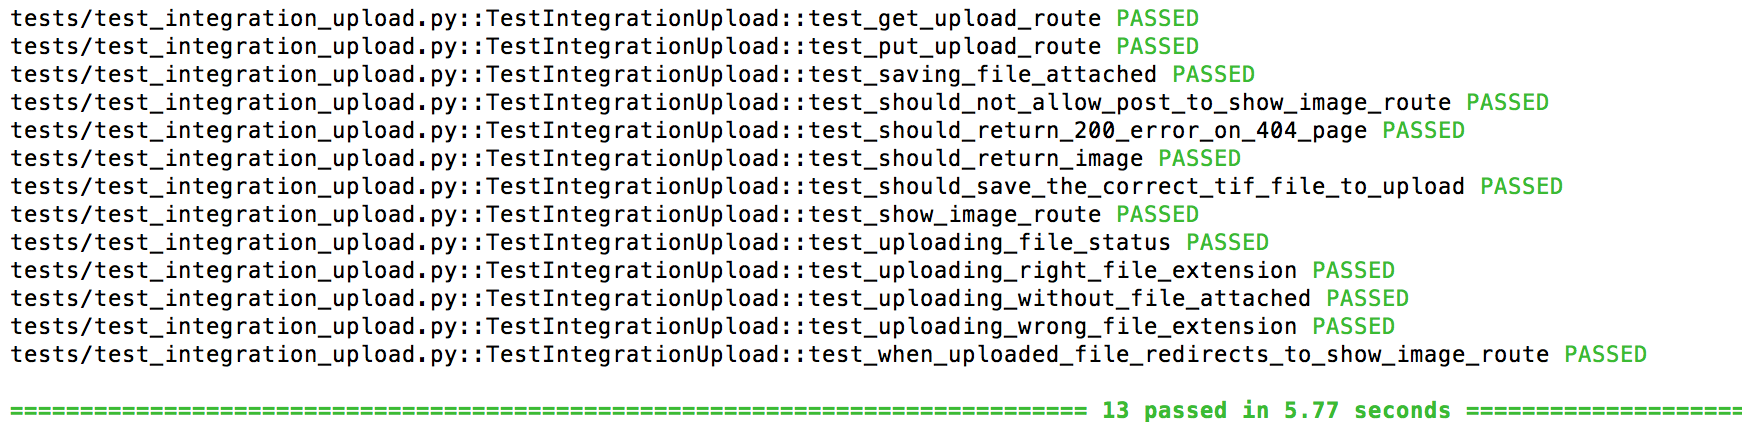
\includegraphics[width=\textwidth]{images/test_integration_upload}
  \caption{Integration tests implemented to ensure that a user can upload their images to the application. }
  \label{fig:integration_upload}
\end{figure}

\section{User}
\begin{figure}[H]
  \centering
  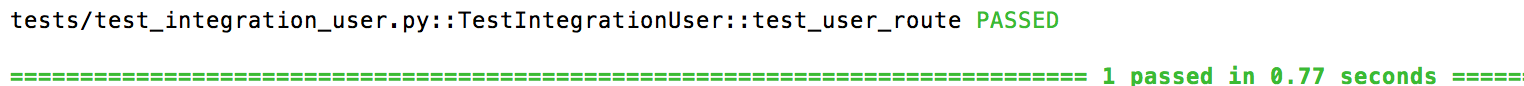
\includegraphics[width=\textwidth]{images/test_integration_user}
  \caption{Integration tests implemented the user route is working correctly and a the user gets added to the database.}
  \label{fig:integration_user}
\end{figure}

\section{View all notes}
\begin{figure}[H]
  \centering
  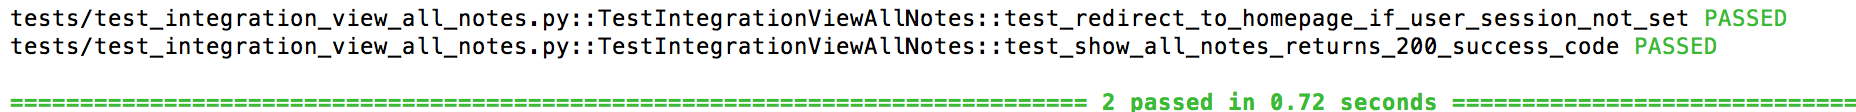
\includegraphics[width=\textwidth]{images/test_integration_view_all_notes}
  \caption{Integration tests to make sure the view all notes url is working and getting the appropriate notes from the database.}
  \label{fig:integration_view_all_notes}
\end{figure}


\section{User tests}
